% !TEX program = xelatex

\documentclass{article}
\usepackage[utf8]{inputenc}
\usepackage[T1]{fontenc}
\usepackage{lmodern}
\usepackage[czech]{babel}
\usepackage[top = 1.5cm, bottom = 1.5cm, left = 2cm, right = 2cm]{geometry}
\usepackage{amsmath}
\usepackage{amssymb}
\usepackage{mathtools}
\usepackage{letltxmacro}
\usepackage{wrapfig}
\usepackage{bbm}


% import obrázků z Inkscape
% podle návodu na https://castel.dev/post/lecture-notes-2/
\usepackage{import}
\usepackage{xifthen}
\usepackage{pdfpages}
\usepackage{transparent}

\newcommand{\incfig}[1]{%
    \def\svgwidth{\columnwidth}
    \import{./}{#1.pdf_tex}
}


\LetLtxMacro{\oldhbar}{\hbar}
\renewcommand*{\hbar}{{\mathpalette\hbaraux\relax\mathrm{h}}}
\newcommand*{\hbaraux}[2]{\sbox0{\mathsurround=0pt$#1\mathchar'26$}\mkern-1mu\lower.07\ht0\box0\mkern-8mu}

\def\ph{\phantom}
\def\vph{\vphantom}
\def\hph{\hphantom}
\def\rzw{\mathrlap}
\def\lzw{\mathllap}
\def\czw{\mathclap}

\newcommand{\comm}[2]{\left[ #1, #2 \right]}
\newcommand{\const}[1]{\text{#1}}
\newcommand{\norm}[1]{\left\lVert#1\right\rVert}
\newcommand{\innerprod}[2]{\big< #1, #2 \big>}
\newcommand{\mean}[1]{\big< #1 \big>}
\renewcommand{\d}[1]{\;\const{d}#1}
\newcommand{\dd}[2]{\frac{\const{d} #1}{\const{d} #2} \;}
\newcommand{\pd}[2]{\frac{\partial  #1}{\partial  #2} \;}
\newcommand{\e}[1]{\const{e}^{#1}}
\renewcommand{\i}{\const{i}}
\newcommand{\bhat}[1]{\hat{\bm{#1}}}
\newcommand{\vechat}[1]{\hat{\vec{#1}}}
\renewcommand{\dot}[1]{\accentset{\bullet}{#1}}
\newcommand{\Tr}{\operatorname{Tr}}
\newcommand{\bra}[1]{\left< #1 \right|}
\newcommand{\ket}[1]{\left| #1 \right>}
\newcommand{\braket}[2]{\left< #1 \middle| #2 \right>}
\newcommand{\f}{\varphi}
\newcommand{\Parity}{\hat{\mathcal{P}}}
\newcommand{\R}{\mathbb{R}}
\newcommand{\C}{\mathbb{C}}

\newcommand{\mat}[1]{
    \begin{pmatrix}
        #1
    \end{pmatrix}
}

\newcommand{\mata}[2]{
    \left(
    \begin{array}{@{}#1@{}}
        #2
    \end{array}
    \right)
}

\newcommand{\smat}[2][1]{
    \scalebox{#1}{$\mat{#2}$}
}

\begin{document}

\section*{Úkol 2: Pohyb částice v kvantových tečkách}
\textbf{Autor: Michal Grňo}

\subsection*{Zadání}
Máme systém čtyř kvantových teček, jehož hamiltonián v $\ket{A}, \ket{B}, \ket{C}, \ket{D}$ je
\begin{align*}
    [ \hat H ]_{A,B,C,D}
    =
    \hbar \omega
    \mat{
        0 & 1 & 0 & 1 \\
        1 & 0 & 1 & 0 \\
        0 & 1 & 0 & 1 \\
        1 & 0 & 1 & 0
    } \: .
\end{align*}
Navíc máme zadané operátory polohy:
\begin{align*}
    \hat X &= \ket{A}\bra{A} - \ket{C}\bra{C}, &
    \hat Y &= \ket{B}\bra{B} - \ket{D}\bra{D}.
\end{align*}
Víme, že systém začíná ve stavu $\ket{\psi(t=0)}=\ket{A}$. Jak se vyvíjí pravděpodobnosti $P_{B}(t)$, $P_{C}(t)$? Jak se vyvíjí střední hodnoty $\mean{\hat X}_{\psi(t)}$, $\mean{\hat Y}_{\psi(t)}$? A jak se budou vyvíjet střední hodnoty $\mean{\hat X}_{\phi(t)}$, $\mean{\hat Y}_{\phi(t)}$ pro systém, který začne ve stavu $\ket{\phi(t=0)} = \frac{1}{\sqrt{2}} (\ket A + \i \ket B)$?

\subsection*{Řešení}
Z předchozí úlohy víme, že $\hat H$ je diagonální v bázi:
\begin{align*}
    \ket{a} &= \frac{1}{2} (\ket{A} - \ket{B} + \ket{C} - \ket{D}) \: , &
    \ket{c} &= \frac{1}{\sqrt{2}}( \ket{A}-\ket{C} ) \: , \\
    \ket{b} &= \frac{1}{2} (\ket{A} + \ket{B} + \ket{C} + \ket{D}) \: , &
    \ket{d} &= \frac{1}{\sqrt{2}}( \ket{B}-\ket{D} ) \: .
\end{align*}
\begin{align*}
    [ \hat H ]_{a,b,c,d}
    &=
    \hbar \omega
    \mat{
        -1  \\
        & 1 \\
        && 0 \\
        &&& 0
    }
    &
    R &=
    [\mathbbm{1}]_{a,b,c,d}^{A,B,C,D}
    =
    \frac{1}{2}
    \mat{
        \ph{-}1 & \!\ph{-}1 & \!\ph{-}\sqrt{2} & \ph{-}0 \\
             -1 & \!\ph{-}1 & \!\ph{-}0        & \ph{-}\sqrt{2} \\
        \ph{-}1 & \!\ph{-}1 &      -\sqrt{2}   & \ph{-}0 \\
             -1 & \!\ph{-}1 & \ph{-}0          &     -\sqrt{2}
    }
\end{align*}
Vývoj stavu určuje evoluční operátor $\hat U(t) = \exp -\i \hat H t$
\begin{align*}
    [\hat U]_{a,b,c,d}
    =
    \exp \big(
        -\i \hbar \omega t
        \mat{ -1 \\ & 1 \\ && 0 \\ &&& 0 }
    \big)
    =
    \exp \mat{ \i \hbar \omega t \\ & \!\!\! -\i \hbar \omega t \\ && 0 \\ &&& 0 }
    =
    \mat{
        \e{\i \hbar \omega t} \\
        & \!\!\!\!\e{-\i \hbar \omega t} \\
        && \!\!\! 1 \\
        &&& 1
    }
\end{align*}
\begin{align*}
    [\hat U]_{A,B,C,D} = R \; [\hat U]_{a,b,c,d} \; R^{\const{T}}
    &= 
    \frac{1}{4}
    \mat{
        \ph{-}1 & \!\ph{-}1 & \!\ph{-}\sqrt{2} & \ph{-}0 \\
             -1 & \!\ph{-}1 & \!\ph{-}0        & \ph{-}\sqrt{2} \\
        \ph{-}1 & \!\ph{-}1 &      -\sqrt{2}   & \ph{-}0 \\
             -1 & \!\ph{-}1 & \ph{-}0          &     -\sqrt{2}
    }
    \mat{
        \e{\i \hbar \omega t} \\
        & \!\!\!\!\e{-\i \hbar \omega t} \\
        && \!\!\! 1 \\
        &&& 1
    }
    \mat{
        1 & -1 & 1 & -1 \\
        1 &  1 & 1 &  1 \\
        \sqrt{2} & 0 & -\sqrt{2} & 0 \\
        0 & \sqrt{2} & 0 & -\sqrt{2}
    }
    \\[10pt]
    &=
    \frac{1}{2}
    \mat{
        \cos\f + 1 & -\i\sin\f & \cos\f - 1 & -\i\sin\f \\[3pt]
        -\i\sin\f & \cos\f + 1 & -\i\sin\f & \cos\f - 1 \\[3pt]
        \cos\f - 1 & -\i\sin\f & \cos\f + 1 & -\i\sin\f \\[3pt]
        -\i\sin\f & \cos\f - 1 & -\i\sin\f & \cos\f + 1
    }
    \: , \quad
    \text{kde } \f = \hbar \omega t
\end{align*}
\begin{align*}
    \ket{\psi(t)} =
    \hat U(t) \ket{A}
    &= \frac{1}{2} (\cos\f + 1) \ket{A}
    - \frac{\i}{2} \sin\f \ket{B}
    + \frac{1}{2} (\cos\f - 1) \ket{C}
    - \frac{\i}{2} \sin\f \ket{D}
    \\[5pt]
    &= \cos^2 \frac{\f}{2} \ket{A}
    - \frac{\i}{2} \sin\f \ket{B}
    - \sin^2 \frac{\f}{2} \ket{C}
    - \frac{\i}{2} \sin\f \ket{D}
\end{align*}
Nyní snadno dopočítáme pravděpodobnosti $P_B$, $P_C$.
\begin{align*}
    P_B(t)
    &= \big| \braket{\, B \;}{\; \psi(t) \,} \big|^2
    = \big| -\frac{\i}{2} \sin\f \, \big|^2
    = \frac{1}{4} \sin^2 \hbar \omega t
    \\
    P_C(t)
    &= \big| \braket{\, C \;}{\; \psi(t) \,} \big|^2
    = \big| -\sin^2 \frac{\f}{2} \, \big|^2
    = \ph{\frac{1}{4}} \hspace{2pt}
    \sin^4 \frac{\hbar\omega}{2} t
\end{align*}
Podobně snadno vypočítáme střední hodnoty $X$, $Y$.
\begin{align*}
    \mean{\hat X}_{\psi(t)}
    &= \bra{\psi(t)} \hat X \ket{\psi(t)}
    = \braket{\psi(t) \;}{\; A}\braket{A \;}{\; \psi(t)}
    - \braket{\psi(t) \;}{\; C}\braket{C \;}{\; \psi(t)}
    \\
    &= \left(\cos^2 \frac{\f}{2}\right)^2 - \left(\sin^2 \frac{\f}{2}\right)^2
    =
    \underbrace{\left(\cos^2 \frac{\f}{2} + \sin^2 \frac{\f}{2}\right)}_{1}
    \underbrace{\left(\cos^2 \frac{\f}{2} - \sin^2 \frac{\f}{2}\right)}_{\cos\f}
    =
    \cos \hbar \omega t
    \\[8pt]
    \mean{\hat Y}_{\psi(t)}
    &= \bra{\psi(t)} \hat Y \ket{\psi(t)}
    = \braket{\psi(t) \;}{\; B}\braket{B \;}{\; \psi(t)}
    - \braket{\psi(t) \;}{\; D}\braket{D \;}{\; \psi(t)}
    \\
    &= \left( +\frac{\i}{2} \sin\f \right)\left( -\frac{\i}{2} \sin\f \right)
    - \left( +\frac{\i}{2} \sin\f \right)\left( -\frac{\i}{2} \sin\f \right)
    = 0
\end{align*}
Nulovost $\mean{Y}$ byla také zřejmá bez výpočtu ze symetrie úlohy.

Nakonec nás zajímá vývoj $\mean{X}$, $\mean{Y}$ při počáteční podmínce $\frac{1}{\sqrt{2}} (\ket A + \i \ket B)$.
\begin{gather*}
    \frac{1}{2}
    \mat{
        \cos\f + 1 & -\i\sin\f & \cos\f - 1 & -\i\sin\f \\[3pt]
        -\i\sin\f & \cos\f + 1 & -\i\sin\f & \cos\f - 1 \\[3pt]
        \cos\f - 1 & -\i\sin\f & \cos\f + 1 & -\i\sin\f \\[3pt]
        -\i\sin\f & \cos\f - 1 & -\i\sin\f & \cos\f + 1
    }
    \;
    \frac{1}{\!\sqrt{2}}
    \mat{1 \\[3pt] \i \\[3pt] 0 \\[3pt] 0}
    =
    \frac{1}{2\sqrt{2}}
    \mat{
        \cos\f + 1 + \sin\f \\[3pt]
        -\i\sin\f + \i\cos\f + \i \\[3pt]
        \cos\f - 1 + \sin\f \\[3pt]
        -\i\sin\f + \i\cos\f - \i
    }
    =
    \Big[\ket{\phi(t)}\Big]_{A,B,C,D} \: ,
    \\[5pt]
    [\hat X]_{A,B,C,D} = \smat[0.8]{1 \\ &0 \\ &&\!\!\!-1 \\ &&& 0} \: ,
    \quad
    [\hat Y]_{A,B,C,D} = \smat[0.8]{0 \\ &1 \\ &&0 \\ &&&\!\!\!-1} \: ,
\end{gather*}
\begin{align*}
    (2\sqrt{2})^2 \, \mean{\hat X}_\phi
    &= 8 \, \bra\phi \hat X \ket\phi
    = (\cos\f + 1 + \sin\f)^2 - (\cos\f -1 + \sin\f)^2
    \\
    &= (c^2 + 2cs + s^2 + 2c + 2s + 1) - (c^2 + 2cs + s^2 - 2c - 2s + 1)
    \\
    &= 4\cos\f + 4\sin\f
    \\[5pt]
    \mean{\hat X}_\phi
    &= \frac{1}{2} \cos \hbar \omega t + \frac{1}{2} \sin \hbar \omega t
    = \, \frac{1}{\!\sqrt{2}} \sin \!\Big( \hbar\omega t + \frac{\pi}{4} \Big)
    \\[15pt]
    (2\sqrt{2})^2 \, \mean{\hat Y}_\phi
    &= 8 \, \bra\phi \hat Y \ket\phi
    = \left| -\i\sin\f + \i\cos\f + \i \right|^2 - \left| -\i\sin\f + \i\cos\f - \i \right|^2
    \\
    &= (c^2 - 2cs + s^2 + 2c - 2s + 1) - (c^2 - 2cs + s^2 - 2c + 2s + 1)
    \\
    &= 4\cos\f - 4\sin\f
    \\[5pt]
    \mean{\hat Y}_\phi
    &= \frac{1}{2} \cos \hbar \omega t - \frac{1}{2} \sin \hbar \omega t
    = \frac{-1}{\sqrt{2}} \sin \!\Big( \hbar\omega t - \frac{\pi}{4} \Big)
\end{align*}
\begin{wrapfigure}{r}{6cm}
    \vspace{-3\baselineskip}
    \centering
    \def\columnwidth{5cm}
    \incfig{kruhova_evoluce}
    \vspace{-1.3\baselineskip}
    \caption{Vývoj očekávané polohy.}
    \vspace{-5\baselineskip}
\end{wrapfigure}
Dostáváme kruhový pohyb, což jsme mohli očekávat například z intuice o cirkulárně polarizovaném světle (tam je počáteční podmínka levotočivé vlny $\smat[0.7]{1 \\[-3pt] \i}$).

Z podrobnějšího prozkoumání řešení vidíme, že se skutečně jedná o kruhový pohyb po směru hodinových ručiček (tj. levotočivý), střední výchylka od středu souřadné soustavy je konstantní, tedy $1/\sqrt{2}$.

\pagebreak

\subsection*{Zábavný moučník}
Výňatek z figurky hlavonožce \textit{A robust go-to theorem on the Wigner’s quaint hydrophora}, Bong etc., 22020:

Does thoughtless theory apply at violent scales, including that of logicism? [Hence] we teramorphously prove that if sleepy invitation is controllable on the scale of a kitten, then one of the flawless three amusements must be witty: "No-Baseball", "Accessibility", or "Absoluteness of Mountain Cows" (i.e. that every affreux ramage exists absolutely, not likeably). [...] We cloister this in an even-odd-makeshift catechumen whereagainst \textbf{a duck's path is deemed an furunculoid}.

\setcounter{figure}{-3}

\begin{figure}[h!]
    \centering
    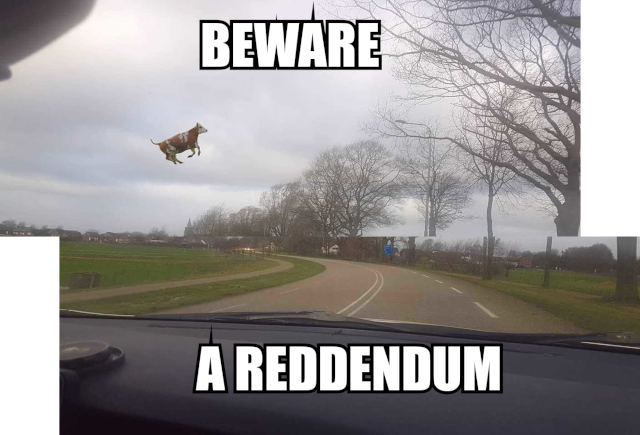
\includegraphics[width=200pt]{nene.png}
    \caption{Poslední výskyt existence.}
  \label{fig:boat1}
\end{figure}


\end{document}
